\documentclass{article}
\usepackage{graphicx}
\usepackage{tikz}
\usepackage{amsmath} 
\usepackage{listings}
\usepackage{color}
\usetikzlibrary{automata, positioning} 
\usetikzlibrary{arrows.meta}

\definecolor{codegreen}{rgb}{0,0.6,0}
\definecolor{codegray}{rgb}{0.5,0.5,0.5}
\definecolor{codepurple}{rgb}{0.58,0,0.82}
\definecolor{backcolour}{rgb}{0.95,0.95,0.92}

\lstdefinestyle{mystyle}{
    backgroundcolor=\color{backcolour},   
    commentstyle=\color{codegreen},
    keywordstyle=\color{magenta},
    numberstyle=\tiny\color{codegray},
    stringstyle=\color{codepurple},
    basicstyle=\ttfamily\footnotesize,
    breakatwhitespace=false,         
    breaklines=true,                 
    captionpos=b,                    
    keepspaces=true,                 
    numbers=left,                    
    numbersep=5pt,                  
    showspaces=false,                
    showstringspaces=false,
    showtabs=false,                  
    tabsize=2
}
\lstset{style=mystyle}

\begin{document}
\begin{titlepage}
    \centering
    \vspace*{1cm}
    \includegraphics[width=4.5cm]{logo_udg.png}\\[1.2cm]
    {\large Universidad de Guadalajara}\\[0.2cm]
    {\large Centro Universitario de Ciencias Exactas e Ingenierías}\\[2.5cm]
    {\LARGE \textbf{Diseño de una Máquina Expendedora usando una MEF con arquitectura Moore}}\\[0.5cm]
    {\large Teoría de la Computación}\\[1cm]
    {\large \textbf{Alumno:} José Luis Chávez Gómez}\\[0.5cm]
    {\large \textbf{Codigo:} 220419709}\\[0.5cm]
    {\large 11 de noviembre del 2026}
    \vfill
\end{titlepage}

\section{Definición formal}
{\large La máquina expendedora se define formalmente como el autómata:} 
{\LARGE \[ M = (Q, \Sigma, \delta, q_0, F) \]} 
{\large donde:}

\begin{itemize}
    \item \textbf{$Q$ (Conjunto de estados):} 
    \begin{itemize}
        \item $q_0$: Estado inicial.
        \item $q_{x, s}$: Estados de acumulación de saldo ($x$ es el productoy $s$ es el dinero).
        \item $q_{entrega}$: Estado de Aceptación.
        \item $q_{error}$: Estado de error.
    \end{itemize}
    
    \item \textbf{$\Sigma$ (Alfabeto):} Productos (a-j) y monedas. \\
    \\ $\Sigma = \{a, b, c, d, e, f, g, h, i, j, 1, 2, 5, 10\}$.
    
    \item \textbf{$q_0$ (Estado inicial):} $q_0$
    
    \item \textbf{$F$ (Estados de aceptación):} $F = \{ q_{x, s} \mid s \ge precio(x) \}$ 
    
    \item \textbf{$\delta$ (Función de transición):} $Q \times \Sigma \to Q$:
    \begin{itemize}
        \item \textbf{Selección de producto:}  $\delta(q_0, x) = q_{x, 0}$ (Pasa a esperar dinero).
        \item \textbf{Acumulación de monedas:} $\delta(q_{x, s}, m) = q_{x, s+m}$ (Suma el valor).
        \item \textbf{Error de selección previa:} $\delta(q_0, m) = q_{error}$ (No se inserta dinero antes del producto).
        \item \textbf{Error de selección doble:}  $\delta(q_{x, s}, y) = q_{error}$ (Solo un producto por transaccion).
    \end{itemize}
\end{itemize}

\section{Diseño de estados}

\begin{itemize}
    \item \textbf{Estado Inicial:}
    \begin{itemize}
        \item $q_0$
    \end{itemize}
    
    \item \textbf{Estados de Selección de Producto:}
    \begin{itemize}
        \item $q_{x, 0}$
    \end{itemize}

    \item \textbf{Estados de Acumulación de Dinero:}
    \begin{itemize}
        \item $q_{x, s}$
    \end{itemize}

    \item \textbf{Estados de Aceptación (Entrega de producto):}
    \begin{itemize}
        \item $q_{entrega, x}$
    \end{itemize}

    \item \textbf{Estado de Error:}
    \begin{itemize}
        \item $q_{error}$: La máquina transita hacia aquí si se violan las reglas:
        \begin{enumerate}
            \item Insertar monedas ($m$) estando en $q_0$.
            \item Seleccionar un segundo producto.
        \end{enumerate}
    \end{itemize}
\end{itemize}

\section{Tabla de transiciones}
$\delta: Q \times \Sigma \to Q$ 

\begin{itemize}
    \item $x$: producto seleccionado ($x \in \{a,b,c,d,e,f,g,h,i,j\}$).
    \item $y$: Cualquier otro producto.
    \item $m$: Cualquier moneda valida (1, 2, 5, 10).
    \item $s$: Saldo actual.
\end{itemize}

\begin{table}[h!]
\centering
\resizebox{\textwidth}{!}{
\begin{tabular}{|c|c|c|c|c|c|c|c|}
\hline
\textbf{$Q$} & \textbf{I ($x$)} & \textbf{I 1} & \textbf{I 2} & \textbf{I 5} & \textbf{I 10} & \textbf{($y$)} \\ \hline
$\rightarrow q_0$ & $q_{x, 0}$ & $q_{error}$ & $q_{error}$ & $q_{error}$ & $q_{error}$ & $q_{error}$ \\ \hline
$q_{x, s}$ & $q_{error}$ & $q_{x, s+1}$ & $q_{x, s+2}$ & $q_{x, s+5}$ & $q_{x, s+10}$ & $q_{error}$ \\ \hline
$q_{error}$ & $q_{error}$ & $q_{error}$ & $q_{error}$ & $q_{error}$ & $q_{error}$ & $q_{error}$ \\ \hline
\end{tabular}
}
\caption{El estado de aceptación $F$ se alcanza cuando $s \ge precio(x)$.}
\end{table}

\textbf{\\[0.25cm]Transiciones:}
\begin{itemize}
    \item \textbf{Validas:} Desde el estado inicial $q_0$, únicamente se acepta una letra ($a-j$).
    \\ Una vez en el estado de acumulación $q_{x, s}$, solo se aceptan números.
    \item \textbf{Invalidas:} Si en $q_0$ se ingresa un número, se transita a $q_{error}$\\ Si durante $q_{x, s}$ se intenta seleccionar otra letra, se transita a $q_{error}$.
\end{itemize}

\section{Diagrama de estados}

\vspace{0.5cm}
\begin{center}
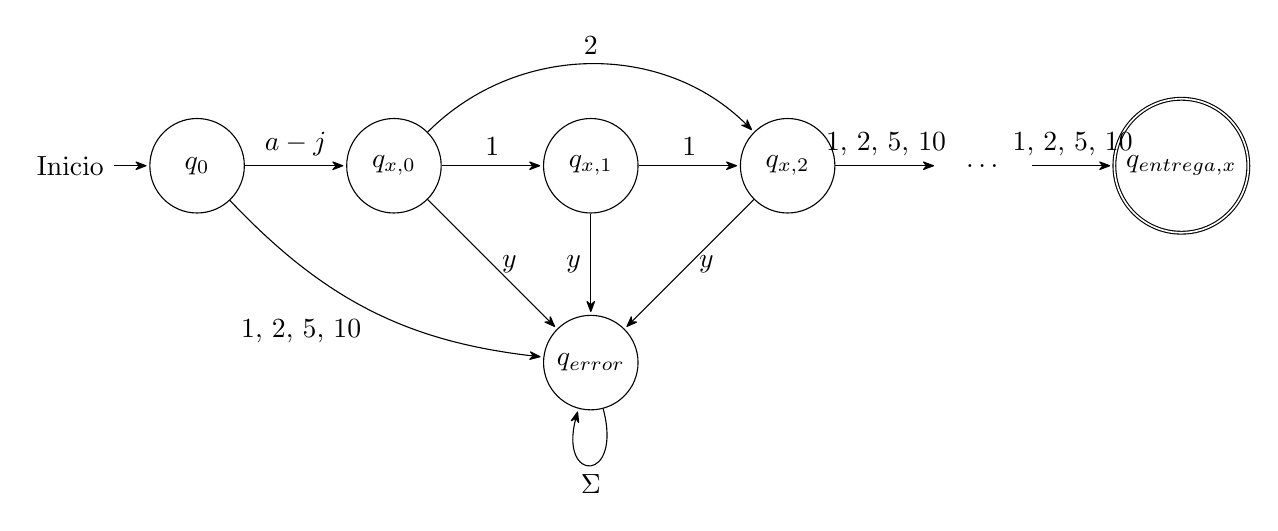
\begin{tikzpicture}[shorten >=1pt, node distance=2.5cm, on grid, >={Stealth[round]}, auto, every state/.style={minimum size=1.2cm}]

  \node[state, initial, initial text=Inicio] (q0) {$q_0$};
  \node[state, right=of q0] (qp0) {$q_{x, 0}$};
  \node[state, right=of qp0] (qp1) {$q_{x, 1}$};
  \node[state, right=of qp1] (qp2) {$q_{x, 2}$};
  \node[state, draw=none, right=of qp2] (dots) {$\dots$};
  \node[state, accepting, right=of dots] (qpf) {$q_{entrega,x}$};

  \node[state, below=2.5cm of qp1] (qerr) {$q_{error}$};

  \path[->]

    (q0) edge node[above] {$a-j$} (qp0)
    
    (qp0) edge node[above] {1} (qp1)
    (qp1) edge node[above] {1} (qp2)
    (qp2) edge node[above] {1, 2, 5, 10} (dots)
    (dots) edge node[above] {1, 2, 5, 10} (qpf)

    (qp0) edge[bend left=45] node[above] {2} (qp2)

    (q0) edge[bend right=20] node[below left] {1, 2, 5, 10} (qerr)
    (qp0) edge node[right] {$y$} (qerr)
    (qp1) edge node[left] {$y$} (qerr)
    (qp2) edge node[right] {$y$} (qerr)

    (qerr) edge[loop below] node {$\Sigma$} (qerr);

\end{tikzpicture}
\end{center}

\section{Validación de cadenas}

\subsection{Cadenas Válidas (Aceptadas)}
\begin{enumerate}
    \item \textbf{Cadena:} \texttt{g, 1, 2} (agua: \$3)
    \begin{itemize}
        \item \textbf{Camino:} $q_0 \xrightarrow{g} q_{agua, 0} \xrightarrow{1} q_{agua, 1} \xrightarrow{2} q_{agua, 3}$
    \end{itemize}
    \item \textbf{Cadena:} \texttt{a, 5, 5} (cocacola: \$10)
    \begin{itemize}
        \item \textbf{Camino:} $q_0 \xrightarrow{a} q_{cocacola, 0} \xrightarrow{5} q_{cocacola, 5} \xrightarrow{5} q_{cocacola, 10}$
    \end{itemize}
    \item \textbf{Cadena:} \texttt{c, 10, 10, 5} (sprite: \$20)
    \begin{itemize}
        \item \textbf{Camino:} $q_0 \xrightarrow{c} q_{sprite, 0} \xrightarrow{10} q_{sprite, 10} \xrightarrow{10} q_{sprite, 20} \xrightarrow{5} q_{sprite, 25}$
    \end{itemize}
    \item \textbf{Cadena:} \texttt{j, 10, 10, 10} (topochico: \$30)
    \begin{itemize}
        \item \textbf{Camino:} $q_0 \xrightarrow{j} q_{topochico, 0} \xrightarrow{10} q_{topochico, 10} \xrightarrow{10} q_{topochico, 20} \xrightarrow{10} q_{topochico, 30}$
    \end{itemize}
    \item \textbf{Cadena:} \texttt{d, 5} (squirt: \$4)
    \begin{itemize}
        \item \textbf{Camino:} $q_0 \xrightarrow{d} q_{squirt, 0} \xrightarrow{5} q_{squirt, 5}$
    \end{itemize}
\end{enumerate}

\subsection{Cadenas Inválidas (Rechazadas)}
\begin{enumerate}
    \item \textbf{Cadena:} \texttt{1, 2, a}
    \begin{itemize}
        \item \textbf{Camino:} $q_0 \xrightarrow{1} q_{error} \xrightarrow{2} q_{error} \xrightarrow{a} q_{error}$
    \end{itemize}
    \item \textbf{Cadena:} \texttt{b, c, 10}
    \begin{itemize}
        \item \textbf{Camino:} $q_0 \xrightarrow{b} q_{fanta, 0} \xrightarrow{c} q_{error} \xrightarrow{10} q_{error}$
    \end{itemize}
    \item \textbf{Cadena:} \texttt{f, 10, 5} (pepsi: \$17)
    \begin{itemize}
        \item \textbf{Camino:} $q_0 \xrightarrow{f} q_{pepsi, 0} \xrightarrow{10} q_{pepsi, 10} \xrightarrow{5} q_{pepsi, 15}$
    \end{itemize}
    \item \textbf{Cadena:} \texttt{g, g}
    \begin{itemize}
        \item \textbf{Camino:} $q_0 \xrightarrow{g} q_{agua, 0} \xrightarrow{g} q_{error}$
    \end{itemize}
    \item \textbf{Cadena:} \texttt{h, 10, 10, 5, 1, 1} (sangria: \$28)
    \begin{itemize}
        \item \textbf{Camino:} $q_0 \xrightarrow{h} q_{sangria, 0} \xrightarrow{10, 10, 5, 1, 1} q_{sangria, 27}$
    \end{itemize}
\end{enumerate}

\section{Implementación}
El modelo matemático se implementó en C 
\lstinputlisting[language=C, caption={Código fuente en C de la Máquina Expendedora}]{machine.c}

\section{Conclusión}
Esta actividad me permitio aplicar los conocimientos acerca de maquinas de estado, sus transiciones y estados, automatas, tablas de transicion, diagrama de estados, y arquitectura moore. Si soy honesto, se me dificulta comprender e intrepretar la definicion matematica, sin embargo el ejemplo que hice sobre una maquina dispensadora de productos, me dejo entender mas, por lo que considero satisfactorio el resultado obtenido.

\section{Referencias bibliográficas}
Gómez Andrade, A. (2018). \textit{Teoría de la Computación: Máquinas abstractas y modelos matemáticos.} Universidad de Guadalajara.

\end{document}